\documentclass[10pt,winfonts,fancyhdr,hyperref,UTF8]{ctexrep}
\usepackage{indentfirst} 
\usepackage{fontspec}
\usepackage{titlesec}
\usepackage{xeCJK}
\usepackage{graphicx}
\usepackage{ifthen}
\usepackage{color,fancyvrb}
\usepackage{listings}
\usepackage{syntonly}
\usepackage{makeidx}
\usepackage[hidelinks, colorlinks=true]{hyperref}
\usepackage{algorithm}
\usepackage{algpseudocode}
\usepackage{amssymb}
\usepackage{multirow}
\usepackage{ulem}
\usepackage{diagbox}
\makeatletter
%LeetCode Setting
\usepackage[centering,paperwidth=180mm,paperheight=230mm,%
body={390pt,530pt},marginparsep=10pt,marginpar=50pt]{geometry}
\usepackage{color}
\usepackage{enumitem}
\usepackage{fancyvrb}
\usepackage[bottom,perpage,symbol*]{footmisc}
\usepackage{graphicx}
\usepackage[hidelinks]{hyperref}
\usepackage{makeidx}
\usepackage[toc]{multitoc}
\usepackage{pifont}
\usepackage{underscore}
\usepackage{amsmath}

\DefineFNsymbols*{chinese}{{\ding{172}}{\ding{173}}{\ding{174}}{\ding{175}}%
{\ding{176}}{\ding{177}}{\ding{178}}{\ding{179}}{\ding{180}}{\ding{181}}}
\setfnsymbol{chinese}

\hypersetup{bookmarksnumbered=true,bookmarksdepth=2}

\CTEXsetup[number={\thechapter}]{chapter}
\CTEXsetup[format+={\raggedleft}]{chapter}
\CTEXsetup[beforeskip={10pt}]{chapter}
\CTEXsetup[afterskip={30pt}]{chapter}
\def\CTEX@chapter@aftername{\par} % \CTEXsetup[aftername={\par}]{chapter}
\CTEXsetup[format+={\raggedright}]{section}
\CTEXsetup[beforeskip={-3.0ex plus -1ex minus -.2ex}]{section}
\CTEXsetup[afterskip={2.3ex plus .2ex minus 0.2ex}]{section}

\renewcommand \thefigure{\thechapter-\arabic{figure}}
\renewcommand \thetable{\thechapter-\arabic{table}}

\newcommand\figcaption[1]{\def\@captype{figure}\caption{#1}}
\newcommand\tabcaption[1]{\def\@captype{table}\caption{#1}}

\long\def\@caption#1[#2]#3{%
  \addcontentsline{\csname ext@#1\endcsname}{#1}%
    {\protect\numberline{\csname fnum@#1\endcsname}{ \ignorespaces #2}}% change "the" to "fnum@"
    \normalsize
    \@makecaption{\csname fnum@#1\endcsname}{\ignorespaces #3}}

\long\def\@makecaption#1#2{%
  \vskip\abovecaptionskip
  \sbox\@tempboxa{#1\quad#2}%
  \ifdim \wd\@tempboxa >\hsize
    #1\quad#2\par
  \else
    \global \@minipagefalse
    \hb@xt@\hsize{\hfil\box\@tempboxa\hfil}%
  \fi
  \vskip\belowcaptionskip}

\setlength\abovecaptionskip{0pt}
  
\setmainfont{Times New Roman}
%\setmainfont{Linux Libertine}
%\setmainfont{TeX Gyre Pagella}
\newfontfamily\urlfont{Times New Roman}
%\setmonofont[AutoFakeBold=1.6,AutoFakeSlant=0.17,Mapping=tex-text-tt]{Inconsolata}
\setCJKfamilyfont{zhyou}{YouYuan}

\newcommand{\fn}[1]{\texttt{#1}}
\newcommand{\sfn}[1]{\texttt{\small #1}}
\newcommand{\kw}[1]{\textsf{#1}}
\newcommand{\myurl}[1]{{\urlfont #1}}
\newcommand{\mpar}[1]{\marginpar[\hfill\kaishu #1]{\kaishu #1}}
\newcommand{\mn}[1]{\texttt{\bs #1}}
\renewcommand{\today}{\the\year-\the\month-\the\day}
\newcommand\bs{\textbackslash}
\newcommand{\code}[1]{\small{\fontspec{Latin Modern Mono} #1}}

\newcommand\begindot{\begin{itemize}
[itemsep=2pt plus 2pt minus 2pt,%
topsep=3pt plus 2pt minus 2pt,%
parsep=0pt plus 2pt minus 2pt]}
\newcommand\myenddot{\end{itemize}}

\newcommand\beginnum{\begin{enumerate}
[itemsep=2pt plus 2pt minus 2pt,%
topsep=3pt plus 2pt minus 2pt,%
parsep=0pt plus 2pt minus 2pt]}
\newcommand\myendnum{\end{enumerate}}

\DefineVerbatimEnvironment%
  {Code}{Verbatim}
  {fontsize=\small,baselinestretch=0.9,xleftmargin=3mm}

\raggedbottom
%\setlength{\parskip}{1ex plus .5ex minus .5ex}

\def\FV@SetLineWidth{%
  \if@FV@ResetMargins\else
    \advance\leftmargin\@totalleftmargin
  \fi
  \advance\leftmargin\FV@XLeftMargin\relax
  \advance\rightmargin\FV@XRightMargin\relax
  \linewidth\hsize
  %\advance\linewidth-\leftmargin
  %\advance\linewidth-\rightmargin
  \hfuzz\FancyVerbHFuzz\relax}


\def\FV@SingleFrameLine#1{%
%% DG/SR modification end
  \hbox to\z@{%
    %\kern\leftmargin
%% DG/SR modification begin - Jun. 22, 1998
    \ifnum#1=\z@
      \let\FV@Label\FV@LabelBegin
    \else
      \let\FV@Label\FV@LabelEnd
    \fi
    \ifx\FV@Label\relax
%% DG/SR modification end
      \FancyVerbRuleColor{\vrule \@width\linewidth \@height\FV@FrameRule}%
%% DG/SR modification begin - Jun. 22, 1998
    \else
      \ifnum#1=\z@
        \setbox\z@\hbox{\strut\enspace\urlfont\FV@LabelBegin\strut}%
      \else
        \setbox\z@\hbox{\strut\enspace\urlfont\FV@LabelEnd\strut}%
      \fi
      \@tempdimb=\dp\z@
      \advance\@tempdimb -.5\ht\z@
      \@tempdimc=\linewidth
      \advance\@tempdimc -\wd\z@
      %\divide\@tempdimc\tw@
      \ifnum#1=\z@              % Top line
        \ifx\FV@LabelPositionTopLine\relax
          \FancyVerbRuleColor{\vrule \@width\linewidth \@height\FV@FrameRule}%
        \else
          \FV@FrameLineWithLabel
        \fi
      \else                     % Bottom line
        \ifx\FV@LabelPositionBottomLine\relax
          \FancyVerbRuleColor{\vrule \@width\linewidth \@height\FV@FrameRule}%
        \else
          \FV@FrameLineWithLabel
        \fi
      \fi
    \fi
%% DG/SR modification end
    \hss}}


%% DG/SR modification begin - May. 19, 1998
\def\FV@FrameLineWithLabel{%
  \ht\z@\@tempdimb\dp\z@\@tempdimb%
  \FancyVerbRuleColor{%
    \raise 0.5ex\hbox{\vrule \@width\@tempdimc \@height\FV@FrameRule}%
    \raise\@tempdimb\box\z@}}
%% DG/SR modification end


\def\FV@EndListFrame@Lines{%
  \begingroup
    %\vskip 0.5ex
    \baselineskip\z@skip
    \kern\FV@FrameSep\relax
%% DG/SR modification begin - May. 19, 1998
%%    \FV@SingleFrameLine
    \FV@SingleFrameLine{\@ne}%
%% DG/SR modification end
  \endgroup}

\newskip\mytopsep
\setlength{\mytopsep}{4pt plus 2pt minus 3pt}

\def\FV@ListVSpace{%
  \@topsepadd\mytopsep
  \if@noparlist\advance\@topsepadd\partopsep\fi
  \if@inlabel
    \vskip\parskip
  \else
    \if@nobreak
      \vskip\parskip
      \clubpenalty\@M
    \else
      \addpenalty\@beginparpenalty
      \@topsep\@topsepadd
      \advance\@topsep\parskip
      \addvspace\@topsep
    \fi
  \fi
  %\showthe \@topsepadd
  %\showthe \topsep
  %\showthe \partopsep
  %\showthe \parskip
  \global\@nobreakfalse
  \global\@inlabelfalse
  \global\@minipagefalse
  \global\@newlistfalse}

\def\FV@EndList{%
  \FV@ListProcessLastLine
  \FV@EndListFrame
  %\showthe \@topsepadd
  \@endparenv
  \endgroup
  \@endpetrue}

\def\theFancyVerbLine{\sffamily\scriptsize\arabic{FancyVerbLine}}

\DefineVerbatimEnvironment%
  {Codex}{Verbatim}
  {fontsize=\small,baselinestretch=0.9,xleftmargin=3mm,%
  frame=lines,labelposition=all,framesep=5pt}

\DefineVerbatimEnvironment%
  {Code}{Verbatim}
  {fontsize=\small,baselinestretch=0.9,xleftmargin=3mm}

\makeindex

%Other settings:
\lstset{%  
  alsolanguage=Java,  
  language={C++},
  tabsize=4, %  
  frame=shadowbox, %把代码用带有阴影的框圈起来  
  commentstyle=\color{red!50!green!50!blue!50},%浅灰色的注释  
  rulesepcolor=\color{red!20!green!20!blue!20},%代码块边框为淡青色  
  keywordstyle=\color{blue!90}\bfseries, %代码关键字的颜色为蓝色,粗体  
  showstringspaces=false,%不显示代码字符串中间的空格标记  
  stringstyle=\ttfamily, % 代码字符串的特殊格式  
  keepspaces=true, %  
  breakindent=22pt, %  
  numbers=left,%左侧显示行号 往左靠,还可以为right,或none,即不加行号  
  stepnumber=1,%若设置为2,则显示行号为1,3,5,即stepnumber为公差,默认stepnumber=1  
  %numberstyle=\tiny, %行号字体用小号  
  numberstyle={\color[RGB]{0,192,192}\tiny} ,%设置行号的大小,大小有tiny,scriptsize,footnotesize,small,normalsize,large等  
  numbersep=8pt,  %设置行号与代码的距离,默认是5pt  
  basicstyle=\footnotesize, % 这句设置代码的大小  
  showspaces=false, %  
  flexiblecolumns=true, %  
  breaklines=true, %对过长的代码自动换行  
  breakautoindent=true,%  
  breakindent=4em, %  
  aboveskip=1em, %代码块边框  
  tabsize=2,  
  showstringspaces=false, %不显示字符串中的空格  
  backgroundcolor=\color[RGB]{245,245,244},   %代码背景色  
}















\makeatother
%\graphicspath{{images/}}

\usepackage{tikz}
\usetikzlibrary{calc}
\usetikzlibrary{fit}
\usetikzlibrary{positioning}
\usepgflibrary{plotmarks}

\usetikzlibrary{shapes.geometric}

\CustomVerbatimEnvironment{shellcmd}{Verbatim}
{frame=single,rulecolor=\color{blue},framerule=3pt,framesep=1pc,fillcolor=\color{yellow}}

\newcommand{\bookname}{TechNotes}
\renewcommand{\contentsname}{Frameworks} 

\title{\sffamily Frameworks}
\date{\today}
\setcounter{tocdepth}{1}
\setcounter{chapter}{7}

\begin{document}

%\maketitle
\tableofcontents


%TOADD
%!Mode:: "TeX:UTF-8"
 \chapter{Unix编程接口}

\input{Frameworks/bgmanagement.tex}
%!Mode:: "TeX:UTF-8"

\section{Linux Bonding}


Linux的多网卡绑定技术是在网卡驱动程序之上、数据链路层之下实现的一个虚拟层,它将多个网卡虚拟成一块虚拟网卡,所以多网卡绑定驱动程序实际上是一种中间驱动程序,是基本驱动程序与网络协议栈之间的接口。


\begin{figure}
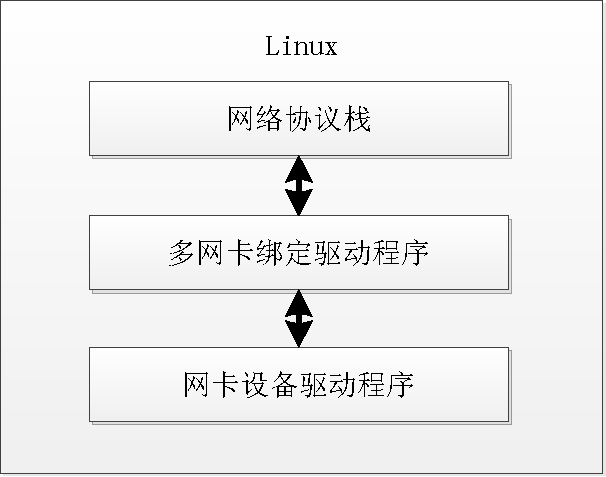
\includegraphics[keepaspectratio,width=0.4\paperwidth]{Pictures/LinuxBondingDriver.pdf} 
\caption{Linux多网卡绑定原理图}
 \label{fig:LinuxBondingDriver}
\end{figure}



目前Linux现有的多网卡绑定驱动共有七种传输模式(算法),依次是:轮转模式、热备份模式、异或模式、广播模式、动态链路聚合模式、自适应传输负载平衡模式、自适应负载平衡模式。\textbf{其中最常用的是模式0、1和6。}

在轮转算法中所有优先级相同的网卡设备维持在一个循环队列中,队列的每个节点(网卡)具有相同的地位,多网卡绑定驱动在这些网卡设备中顺序轮流选择,队列中所有的成员公平分享所有的传输任务。轮转算法的适用面最广,轮转模式适用于绑定驱动中所有节点的处理能力和性能均相同的情况,如适用相同类型的网卡。它的算法思想虽然很简单,但传输能力和传输效率是最好的,不过需要交换机支持,如果交换机未配置链路聚合,则会发生MAC地址表的动荡,在配置了链路聚合后不会出现,发出数据包的MAC为虚拟网卡Bond0的MAC,限制了它的一些应用场合。

模式1的热备份算法可以用来提高服务器的高可用性,在主网卡失效的情况下,备用网卡可以接替主网卡继续工作,但是网卡的利用率只有1/N,效率较低。
    
模式6的平衡负载模式,有自动备援,无需交换机特殊配置,即可实现负载均衡,它们的动态负载均衡方式可以根据绑定设备中网卡的负载状态来动态的分配传输任务,主要适用于服务器拥有四块及四块以上网卡的情况。

%!Mode:: "TeX:UTF-8"
\section{守护进程}

\textbf{守护进程是脱离于终端并且在后台运行的进程}。
守护进程脱离于终端是为了避免进程在执行过程中的信息在任何终端上显示并且进程也不会被任何终端所产生的终端信息所打断。

守护进程,也就是通常说的Daemon进程,是Linux中的后台服务进程。它是一个生存期较长的进程,通常独立于控制终端并且周期性地执行某种任务或等待处理某些发生的事件。守护进程常常在系统引导装入时启动,在系统关闭时终止。Linux系统有很多守护进程,大多数服务都是通过守护进程实现的,同时,守护进程还能完成许多系统任务,例如,作业规划进程crond、打印进程lqd等(这里的结尾字母d就是Daemon的意思)。

Linux守护进程包括:init(系统守护进程,启动各运行层次的系统服务),keventd(为在内核中运行scheduled function提供进程上下文),kapmd(高级电源管理),kswapd(页面交换守护进程),pdflush(内存达到下限时冲洗脏缓冲区),kupdated(定期冲洗脏缓冲区)等。

常见的服务Deamon包括:
\begin{description}
\item[atd and crond]: Task scheduler daemons
\item[bootparmd and dhcpd]: Dynamic Host Configuration Protocol and Internet Bootstrap Protocol servers
\item[fingerd]: Finger server。Finger是UNIX系统中用于查询用户情况的实用程序(dos系统也包含此命令)。UNIX系统保存了每个用户的详细资料,包括E-mail地址、帐号,在现实生活中的真实姓名、登录时间、有没有未阅读的信件,最后一次阅读E-mail的时间以及外出时的留言等资料。当你用Finger命令查询时,系统会将上述资料一一显示在你有终端或计算机上。
\item[ftpd]: File Transfer Protocol (FTP) server
\item[httpd]: Hypertext Transfer Protocol (HTTP) daemon (web server)
\item[identd]: Provides the identity of a user of a particular TCP connection
\item[inetd and xinetd]: Internet Superserver daemon
\item[named]: A Domain Name System (DNS) server daemon
\item[nfsd]: Network File System (NFS) daemon
\item[ntpd]: Network Time Protocol (NTP) service daemon
\item[portmap, rpcbind]: SunRPC port mapper,将RPC程序号映射为网络端口号。
\item[mysqld, postgresql]: Database server daemons
\item[routed, gated]: Manages routing tables
\item[nfsd, mountd, statd]: Part of typical Network File System implementation。mount协议是NFS协议的一部分。
\item[rwhod]: Maintains the database used by the rwho and ruptime tools
\item[sendmail, postfix]: mail transfer agent daemons
\item[snmpd]: Simple Network Management Protocol Daemon
\item[syslogd]: 为各程序提供系统日志功能。
\item[telnetd and sshd]: Telnet and Secure Shell server daemons
\item[ypbind]: A bind server for Network Information Service ("Yellow Pages")
\item[cupsd]: 打印假脱机进程,处理系统提出的所有打印请求。

\end{description}



守护进程创建过程:
\begin{enumerate}
  \item 创建子进程,父进程退出。在Linux中父进程先于子进程退出会造成子进程成为孤儿进程,而每当系统发现一个孤儿进程时,就会自动由1号进程(init)收养它,这样,原先的子进程就会变成init进程的子进程。
  \item 脱离控制终端、登录会话和进程组。由于在调用了fork函数时,子进程全盘拷贝了父进程的会话期、进程组、控制终端等,虽然父进程退出了,但会话期、进程组、控制终端等并没有改变,因此,这还不是真正意义上的独立开来,而setsid函数能够使进程完全独立出来,从而摆脱其他进程的控制。为禁止子进程重新打开控制终端,可以再次调用fork使进程不再成为会话组长:\verb$if(pid=fork()) exit(0);$。
  \item 改变工作目录。一般需要将工作目录改变到根目录(\verb$chdir("/")$) 。
    对于需要转储核心,写运行日志的进程将工作目录改变到特定目录如/tmp。
  \item 重设文件权限掩码。进程从创建它的父进程那里继承了文件创建掩模。它可能修改守护进程所创建的文件的存取位。为防止这一点,将文件创建掩模清除:\verb$umask(0);$。
  \item 关闭文件描述符。
  \item 设置信号处理。如SIGCHLD信号(非必须)。
\end{enumerate}

以下是APUE给出的守护进程创建实例:
\begin{lstlisting}[language=C]
#include "apue.h"
#include <syslog.h>
#include <fcntl.h>
#include <sys/resource.h>

void
daemonize(const char *cmd)
{
    int                 i, fd0, fd1, fd2;
    pid_t               pid;
    struct rlimit       rl;
    struct sigaction    sa;
    /*
     * Clear file creation mask.
     */
    umask(0);

    /*
     * Get maximum number of file descriptors.
     */
    if (getrlimit(RLIMIT_NOFILE, &rl) < 0)
        err_quit("%s: can't get file limit", cmd);

    /*
     * Become a session leader to lose controlling TTY.
     */
    if ((pid = fork()) < 0)
        err_quit("%s: can't fork", cmd);
    else if (pid != 0) /* parent */
        exit(0);
        
    setsid();

    /*
     * Ensure future opens won't allocate controlling TTYs.
     */
    sa.sa_handler = SIG_IGN;
    sigemptyset(&sa.sa_mask);
    sa.sa_flags = 0;
    if (sigaction(SIGHUP, &sa, NULL) < 0)
        err_quit("%s: can't ignore SIGHUP");
    if ((pid = fork()) < 0)
        err_quit("%s: can't fork", cmd);
    else if (pid != 0) /* parent */
        exit(0);

    /*
     * Change the current working directory to the root so
     * we won't prevent file systems from being unmounted.
     */
    if (chdir("/") < 0)
        err_quit("%s: can't change directory to /");

    /*
     * Close all open file descriptors.
     */
    if (rl.rlim_max == RLIM_INFINITY)
        rl.rlim_max = 1024;
    for (i = 0; i < rl.rlim_max; i++)
        close(i);

    /*
     * Attach file descriptors 0, 1, and 2 to /dev/null.
     */
    fd0 = open("/dev/null", O_RDWR);
    fd1 = dup(0);
    fd2 = dup(0);

    /*
     * Initialize the log file.
     */
    openlog(cmd, LOG_CONS, LOG_DAEMON);
    if (fd0 != 0 || fd1 != 1 || fd2 != 2) {
        syslog(LOG_ERR, "unexpected file descriptors %d %d %d",
          fd0, fd1, fd2);
        exit(1);
    }
}


    
\end{lstlisting}

%!Mode:: "TeX:UTF-8"
\section{C/C++中的日期和时间}

\subsection{基本常识}

世界标准世界(Coordinated Universal Time, UTC):协调世界时,又称格林威治标准时间(Greenwich Mean Time,GMT)。中国内地的时间与UTC的时差为+8,也就是UTC+8。美国是UTC-5。 

日历时间(Calendar Time):代表从一个日历参考点到此时的时间经过的秒数。日历参考点(Epoch)因编译器而异,如Unix系统通常使用UTC时间1970年元旦零点作为参考点,称作Unix时间或POSIX时间。

时钟计时单元(clock tick, 而不把它叫做时钟滴答次数):一个时钟计时单元的时间长短是由CPU控制的,但一个clock tick未必是CPU的一个时钟周期,而是C/C++的一个基本计时单位。


\subsection{程序时间:毫秒级精度}
time.h提供了如下计时函数clock(),返回从开启这个程序进程到程序中调用该函数时之间的CPU时钟计时单元(clock tick)数,称为挂钟时间(wall-clock):
\begin{lstlisting}[language=C]
clock_t clock(void);
\end{lstlisting}

函数其中clock\_t定义在time.h文件中,经常是long类型。time.h文件还定义了一个常量表示一秒钟会有多少个时钟计时单元: 
\begin{lstlisting}[language=C]
#define CLOCKS_PER_SEC ((clock_t)1000) 
\end{lstlisting}
表达式\verb|clock()/CLOCKS_PER_SEC|返回一个进程自身的运行时间。

\subsection{日历时间:秒级精度}
time.h通过time()函数返回日历时间,为从日历参考点到此时的秒数。
\begin{lstlisting}[language=C]
time_t time(time_t * timer); 
\end{lstlisting}

time\_t定义于time.h中,可能是long型。如果time\_t类型占32位,且日历参考点为Unix时间,则其表示的时间不能晚于2038年1月18日19时14分07秒。一些编译器厂商引入了64位甚至更长的整形数来保存日历时间。比如微软在Visual C++中采用\verb+__time64_t+数据类型来保存日历时间,并通过\verb|_time64()|函数来获得日历时间(而不是通过使用32位字的time()函数),这样就可以通过该数据类型保存3001年1月1日0时0分0秒(不包括该时间点)之前的时间。 

time.h提供difftime函数,实现两个日历时间值的简单相减(虽然返回值被转换为double型),无大用:
\begin{lstlisting}[language=C]
time_t difftime(time_t t1, time_t t2); 
\end{lstlisting}


\subsection{分解时间}

标准C/C++通过time.h定义tm结构保存时间结构: 
\begin{lstlisting}[language=C]
#ifndef _TM_DEFINED 
struct tm { 
int tm_sec; /* 秒 – 取值区间为[0,59] */ 
int tm_min; /* 分 - 取值区间为[0,59] */ 
int tm_hour; /* 时 - 取值区间为[0,23] */ 
int tm_mday; /* 一个月中的日期 - 取值区间为[1,31] */ 
int tm_mon; /* 月份(从一月开始,0代表一月) - 取值区间为[0,11] */ 
int tm_year; /* 年份,其值等于实际年份减去1900 */ 
int tm_wday; /* 星期 – 取值区间为[0,6],其中0代表星期天,1代表星期一,以此类推 */
int tm_yday; /* 从每年的1月1日开始的天数 – 取值区间为[0,365],其中0代表1月1日,1代表1月2日,以此类推 */ 
int tm_isdst; /* 夏令时标识符,实行夏令时的时候,tm_isdst为正。不实行夏令时的进候,tm_isdst为0;不了解情况时,tm_isdst()为负。*/ 
}; 
#define _TM_DEFINED 
#endif 
\end{lstlisting}

ANSI C标准称使用tm结构的这种时间表示为分解时间(broken-down time)。

time.h提供了以下函数实现日历时间和分解时间的相互转换: 
\begin{lstlisting}[language=C]
struct tm *gmtime(const time_t *timer); 
struct tm *localtime(const time_t *timer); 
time_t mktime(struct tm *timeptr); 
\end{lstlisting}

\subsection{时间显示}
asctime函数将tm结构转换为字符串:
\begin{lstlisting}[language=C]
char *asctime(const struct tm *timeptr);
\end{lstlisting}

asctime通过以下格式显示时间:
\begin{verbatim}
星期几 月份 日期 时:分:秒 年\n\0 
例如:Wed Jan 02 02:03:55 1980\n\0 
\end{verbatim}

ctime函数将日历时间转换为字符串,相当于嵌套调用localtime和asctime:
\begin{lstlisting}[language=C]
char * ctime(const time_t *timer); 
\end{lstlisting}

time.h还提供strftime实现更灵活的时间显示格式:
\begin{lstlisting}[language=C]
size_t strftime(char *strDest, size_t maxsize, const char *format, const struct tm *timeptr); 
\end{lstlisting}

strftime()根据format指向字符串中指定的格式命令把timeptr中保存的时间信息放在strDest指向的字符串中,最多向strDest中存放maxsize个字符。该函数返回向strDest指向的字符串中放置的字符数,使用方式类似于snprintf()。关于显示格式,strftime用\%B表示月份,\%G表示年份,等等。

\subsection{POSIX下的时间获取与设置:微秒精度}
sys/time.h提供了以下函数用于时间获取和设置:
\begin{lstlisting}[language=C]
int gettimeofday(struct timeval *tv, struct timezone *tz);
int settimeofday(const struct timeval *tv, const struct timezone *tz);
\end{lstlisting}

其中timeval结构代表自日历参考点以来的时间:

\begin{lstlisting}[language=C]
    struct timeval {
    time_t      tv_sec;     /* seconds */
    suseconds_t tv_usec;    /* microseconds */
    };
\end{lstlisting}

timezone结构定义如下:
\begin{lstlisting}[language=C]
    struct timezone {
    int tz_minuteswest;     /* minutes west of Greenwich */
    int tz_dsttime;         /* type of DST correction */
    };
\end{lstlisting}

timezone结构的使用已经过时,应该设置为NULL。尤其是tz\_dsttime字段,其在内核中的使用被视作bug。

这两个函数调用成功则返回零,失败则返回-1,同时设置errno。



















%!Mode:: "TeX:UTF-8"
 

\section{ELF文件布局}
在ELF格式的可执行文件中,全局内存包括三种:bss、data和rodata。

bss代表Block Storage Start,是指那些没有初始化的和初始化为0的全局变量。
如\verb$int bss_array[1024 * 1024] = {0};$。
变量\verb$bss_array$的大小为4M,而可执行文件的大小只有5K。 
由此可见,bss类型的全局变量只占运行时的内存空间,而\textbf{不占}文件空间。

data指那些初始化过(非零)的非const的全局变量。
如果数据全是零,为了优化考虑,编译器把它当作bss处理。
data类型的全局变量是即占文件空间,又占用运行时内存空间的。
data的例子如:

\verb$int data_array[1024 * 1024] = {1};$


rodata的意义同样明显,ro代表read only,即只读数据(const)。
常量不一定就放在rodata里,有的立即数直接编码在指令里,存放在代码段(.text)中。
对于字符串常量,编译器会自动去掉重复的字符串,保证一个字符串在一个可执行文件(EXE/SO)中只存在一份拷贝。
rodata是在多个进程间是共享的,这可以提高空间利用率。
在有的嵌入式系统中,rodata放在ROM(如norflash)里,运行时直接读取ROM内存,无需要加载到RAM内存中。
把在运行过程中不会改变的数据设为rodata类型的,是有很多好处的:在多个进程间共享,可以大大提高空间利用率,甚至不占用RAM空间。同时由于rodata在只读的内存页面(page)中,是受保护的,任何试图对它的修改都会被及时发现,这可以帮助提高程序的稳定性。

\subsection{ABI}
应用二进制接口(英语:application binary interface,缩写为 ABI)描述了应用程序(或者其他类型)和操作系统之间或其他应用程序的低级接口。

ABI涵盖了各种细节,如:
\begin{itemize}
\item 数据类型的大小、布局和对齐;
\item 调用约定(控制着函数的参数如何传送以及如何接受返回值),例如,是所有的参数都通过栈传递,还是部分参数通过寄存器传递;哪个寄存器用于哪个函数参数;通过栈传递的第一个函数参数是最先push到栈上还是最后;
\item 系统调用的编码和一个应用如何向操作系统进行系统调用;
\item 以及在一个完整的操作系统ABI中,目标文件的二进制格式、程序库等等。
\end{itemize}
一个完整的ABI,像Intel二进制兼容标准(iBCS),允许支持它的操作系统上的程序不经修改在其他支持此ABI的操作系统上运行。

其他的ABI标准化了一些细节,包括C++ 名称修饰 ,和同一个平台上的编译器之间的调用约定,但是不包括跨平台的兼容性。

ABI不同于应用程序接口(API),API定义了源代码和库之间的接口,因此同样的代码可以在支持这个API的任何系统中编译,然而ABI允许编译好的目标代码在使用兼容ABI的系统中无需改动就能运行。 在Unix风格的操作系统中,存在很多运行在同一硬件平台上互相相关但是不兼容的操作系统(尤其是Intel 80386兼容系统)。有一些努力尝试标准化ABI,以减少销售商将程序移植到其他系统时所需的工作。然而,直到现在还没有很成功的例子,虽然Linux标准化工作组正在为Linux做这方面的努力。
%!Mode:: "TeX:UTF-8"
\section{I/O复用}

\subsection{select API}

\begin{lstlisting}[language=C++]
int select(int nfds, fd_set *readfds, fd_set *writefds, 
  fd_set *exceptfds, struct timeval *timeout);
\end{lstlisting}

select对应于内核中的sys\_select调用,sys\_select首先将第二三四个参数指向的fd\_set拷贝到内核,然后对每个被SET的 述符调用进行poll,并记录在临时结果中(fdset),如果有事件发生,select会将临时结果写到用户空间并返回;当轮询一遍后没有任何事件发生时,如果指定了超时时间,则select会睡眠到超时,睡眠结束后再进行一次轮询,并将临时结果写到用户空间,然后返回。

poll本质上和select没有区别,它将用户传入的数组拷贝到内核空间,然后查询每个fd对应的设备状态,如果设备就绪则在设备等待队列中加入一项并继续遍历,如果遍历完所有fd后没有发现就绪设备,则挂起当前进程,直到设备就绪或者主动超时,被唤醒后它又要再次遍历fd。这个过程经历了多次无谓的遍历。
它没有最大连接数的限制,原因是它是基于链表来存储的,但是同样有一个缺点:
大量的fd的数组被整体复制于用户态和内核地址空间之间,而不管这样的复制是不是有意义。
poll还有一个特点是“水平触发”,如果报告了fd后,没有被处理,那么下次poll时会再次报告该fd。

epoll支持水平触发和边缘触发,最大的特点在于边缘触发,它只告诉进程哪些fd刚刚变为就需态,并且只会通知一次。
在前面说到的复制问题上,epoll使用mmap减少复制开销。
还有一个特点是,epoll使用“事件”的就绪通知方式,通过epoll\_ctl注册fd,一旦该fd就绪,内核就会采用类似callback的回调机制来激活该fd,epoll\_wait便可以收到通知


\subsection{epoll相对select优点}
select和epoll这两个机制都是多路I/O机制的解决方案,select为POSIX标准中的,而epoll为Linux所特有的。

传统的select/poll每次调用都会线性扫描全部的集合,导致效率呈现线性下降。
epoll的IO效率不随FD数目增加而线性下降。
如果所有的socket基本上都是活跃的---比如一个高速LAN环境,过多使用epoll,效率相比还有稍微的下降。但是一旦使用idle connections模拟WAN环境,epoll的效率就远在select/poll之上了。

poll的执行分三部分:
(1).将用户传入的pollfd数组拷贝到内核空间,因为拷贝操作和数组长度相关,时间上这是一个O(n)操作
(2).查询每个文件描述符对应设备的状态,如果该设备尚未就绪,则在该设备的等待队列中加入一项并继续查询下一设备的状态。 查询完所有设备后如果没有一个设备就绪,这时则需要挂起当前进程等待,直到设备就绪或者超时。设备就绪后进程被通知继续运行,这时再次遍历所有设备,以查找就绪设备。这一步因为两次遍历所有设备,时间复杂度也是O(n),这里面不包括等待时间.
(3). 将获得的数据传送到用户空间并执行释放内存和剥离等待队列等善后工作,向用户空间拷贝数据与剥离等待队列等操作的的时间复杂度同样是O(n)。


区别(epoll相对select优点)主要有三:
1.select的句柄数目受限,在linux/posix\_types.h头文件有这样的声明:\verb$#define __FD_SETSIZE 1024$表示select最多同时监听1024个fd。而epoll没有,它的限制是最大的打开文件句柄数目。
2.epoll的最大好处是不会随着FD的数目增长而降低效率,在selec中采用轮询处理,其中的数据结构类似一个数组的数据结构,而epoll是维护一个队列,直接看队列是不是空就可以了。epoll只会对"活跃"的socket进行操作---这是因为在内核实现中epoll是根据每个fd上面的callback函数实现的。那么,只有"活跃"的socket才会主动的去调用 callback函数(把这个句柄加入队列),其他idle状态句柄则不会,在这点上,epoll实现了一个"伪"AIO。但是如果绝大部分的I/O都是“活跃的”,每个I/O端口使用率很高的话,epoll效率不一定比select高(可能是要维护队列复杂)。
3.使用mmap加速内核与用户空间的消息传递。无论是select,poll还是epoll都需要内核把FD消息通知给用户空间,如何避免不必要的内存拷贝就很重要,在这点上,epoll是通过内核于用户空间mmap同一块内存实现的。


\subsection{epoll API}

1.
\begin{lstlisting}[language=C++]
int epoll_create(int size);
\end{lstlisting}

创建一个epoll的句柄,size用来告诉内核这个监听的数目最大值。用close()来关闭。

2.
\begin{lstlisting}[language=C++]
//epoll的事件注册函数
int epoll_ctl(int epfd, int op, int fd, 
  struct epoll_event *event);
\end{lstlisting}
第一个参数是epoll\_create()的返回值,第二个参数表示动作,用三个宏来表示:
\begin{verbatim}
EPOLL_CTL_ADD:注册新的fd到epfd中;
EPOLL_CTL_MOD:修改已经注册的fd的监听事件;
EPOLL_CTL_DEL:从epfd中删除一个fd;
\end{verbatim}
第三个参数是需要监听的fd,第四个参数是告诉内核需要监听什么事,数据结构如下:
\begin{lstlisting}[language=C++]
typedef union epoll_data {
      void        *ptr;
      int          fd;
      uint32_t     u32;
      uint64_t     u64;
} epoll_data_t;

struct epoll_event {
    uint32_t events; /* Epoll events */
    epoll_data_t data;/* User data variable */
};
\end{lstlisting}
events可以是以下几个宏的集合:
\begin{lstlisting}[language=C++]
EPOLLIN :可读(包括对端SOCKET正常关闭)
EPOLLOUT:可写
EPOLLPRI:有紧急的数据可读(这里应该表示有带外数据到来)
EPOLLERR:表示对应的文件描述符发生错误
EPOLLHUP:表示对应的文件描述符被挂断
EPOLLET: 设为边缘触发(Edge Triggered)模式,这是相对于水平触发(Level Triggered)来说的
EPOLLONESHOT:只监听一次事件就会把这个fd从epoll的队列中删除
\end{lstlisting}


3.
\begin{lstlisting}[language=C++]
int epoll_wait(int epfd, struct epoll_event *events, 
  int maxevents, int timeout);
\end{lstlisting}
等待事件的产生,类似于select()调用。参数events用来从内核得到事件的集合,maxevents告之内核这个events有多大,这个maxevents的值不能大于创建epoll\_create()时的size,参数timeout是超时时间(毫秒,0会立即返回,-1是永久阻塞)。该函数返回需要处理的事件数目,如返回0表示已超时















%!Mode:: "TeX:UTF-8"
\section{Linux平台C语言获取本机IP}
方法一:通过gethostname和gethostbyname

方法二:getifaddrs函数获取网卡的所有IP地址

方法三: getsockname获取某个连接所使用的本地IP


%!Mode:: "TeX:UTF-8"
\section{Java Frameworks}


\href{https://en.wikipedia.org/wiki/Java_Platform,_Enterprise_Edition}{Java
Platform, Enterprise Edition or Java EE} is a widely used enterprise computing
The platform provides an API and runtime environment for developing and running
enterprise software, including network and web services, and other large-scale, multi-tiered, scalable, reliable, and secure network applications. 
Java EE extends the Java Platform, Standard Edition (Java SE), providing an API for object-relational mapping, distributed and multi-tier architectures, and web services.

The \href{https://en.wikipedia.org/wiki/Spring_Framework}{Spring Framework} is
an application framework and inversion of control (IoC) container for the Java platform.
The framework's core features can be used by any Java application, but there are extensions for building web applications on top of the Java EE platform. 
Although the framework does not impose any specific programming model, 
it has become popular in the Java community as an alternative to, replacement for, or even addition to the Enterprise JavaBeans (EJB) model. 
The Spring Framework is open source.


\href{https://en.wikipedia.org/wiki/Enterprise_JavaBeans}{Enterprise JavaBeans (EJB)} 
is a managed, server software for modular construction of enterprise
software, and one of several Java APIs.
EJB is a server-side software component that encapsulates the business logic of an application.
The EJB specification is a subset of the Java EE specification. 
An EJB web container provides a runtime environment for web related software components, including computer security, Java servlet lifecycle management, transaction processing, and other web services.

The complexity issue continued to hinder EJB's acceptance.
\href{https://en.wikipedia.org/wiki/Hibernate_(framework)}{Hibernate} (for persistence and object-relational mapping) and 
\href{https://en.wikipedia.org/wiki/Spring_Framework}{Spring Framework} (which provided an alternate and far less verbose way to encode
business logic) were created to replace it and grew in popularity, despite
lacking the support of big businesses.


\href{https://en.wikipedia.org/wiki/Hibernate_(framework)}{Hibernate ORM} 
(Hibernate in short) is an object-relational mapping framework for the Java language. 
It provides a framework for mapping an object-oriented domain model to a relational database. 
Hibernate solves object-relational impedance mismatch problems by replacing direct, persistent database accesses with high-level object handling functions.
Hibernate's primary feature is mapping from Java classes to database tables; and
mapping from Java data types to SQL data types. Hibernate also provides data query and retrieval facilities. It generates SQL calls and relieves the developer from manual handling and object conversion of the result set.

\href{https://en.wikipedia.org/wiki/Apache_Struts_2}{Apache Struts 2} is an
open-source web application framework for developing Java EE web applications. 
It uses and extends the Java Servlet API to encourage developers to adopt a model–view–controller (MVC) architecture.
 It favors convention over configuration, is extensible using a plugin architecture, and ships with plugins to support REST, AJAX and JSON.

The integration of Struts, Spring and Hibernate is often abbreviated as
\textbf{SSH}.



\href{https://en.wikipedia.org/wiki/Non-blocking_I/O_(Java)}{Non-blocking I/O}
(usually called \textbf{NIO}, and sometimes called "New I/O") is a collection of
Java programming language APIs that offer features for intensive I/O operations.
It was introduced with the J2SE 1.4 release of Java by Sun Microsystems to complement an existing standard I/O.

\href{https://en.wikipedia.org/wiki/Netty_(software)}{Netty} is a NIO
client-server framework for the development of Java network applications such as protocol servers and clients. 
The asynchronous event-driven network application framework and tools are used to simplify network programming such as TCP and UDP socket servers.
Netty includes an implementation of the reactor pattern of programming.

\href{https://en.wikipedia.org/wiki/Apache_MINA}{Apache MINA} (Multipurpose
Infrastructure for Network Applications) is an open source Java network application framework. MINA can be used to create scalable, high performance network applications. 
MINA provides unified APIs for various transports like TCP, UDP, serial communication. 
It also makes it easy to make an implementation of custom transport type. 
MINA provides both high-level and low-level network APIs.











%!Mode:: "TeX:UTF-8"
\section{Apache Kafka}

\href{https://en.wikipedia.org/wiki/Apache_Kafka}{Apache Kafka} is an
open-source message broker project developed by the Apache Software Foundation written in Scala.


A simple kafka producer in Python using python-kafka package:
\begin{verbatim}
from kafka import KafkaProducer
producer = KafkaProducer(bootstrap_servers='172.30.30.247:9092')
for _ in range(10):
    producer.send('topic_name', b'some_message_bytes') 
\end{verbatim}


%!Mode:: "TeX:UTF-8"
 
\section{进程/线程与CPU核的绑定}
\verb$sched_setaffinity$实现进程与核的绑定。

\begin{lstlisting}[language=C++]
int pthread_setaffinity_np(pthread_t thread, size_t cpusetsize, const  cpu_set_t *cpuset);
int pthread_getaffinity_np(pthread_t thread, size_t cpusetsize, cpu_set_t  *cpuset);
\end{lstlisting}
分别设置和获取线程的亲和性。

\verb$cpu_set_t$类似于select中的\verb$fd_set$可以理解为cpu集,也是通过约定好的宏来进行清除、设置以及判断:
\begin{lstlisting}[language=C++]
//初始化,设为空
void CPU_ZERO (cpu_set_t *set); 
//将某个cpu加入cpu集中 
void CPU_SET (int cpu, cpu_set_t *set); 
//将某个cpu从cpu集中移出 
void CPU_CLR (int cpu, cpu_set_t *set); 
//判断某个cpu是否已在cpu集中设置了 
int CPU_ISSET (int cpu, const cpu_set_t *set); 
\end{lstlisting}

cpu集可以认为是一个掩码,每个设置的位都对应一个可以合法调度的 cpu,而未设置的位则对应一个不可调度的 CPU。
换而言之,线程都被绑定了,只能在那些对应位被设置了的处理器上运行。通常,掩码中的所有位都被置位了,也就是可以在所有的cpu中调度。       
      
以下为测试代码:

\begin{lstlisting}[language=C++]
#define _GNU_SOURCE
#include <stdio.h>
#include <stdlib.h>
#include <string.h>
#include <unistd.h>
#include <pthread.h>
#include <sched.h>

void *myfun(void *arg)
{
    cpu_set_t mask;
    cpu_set_t get;
    char buf[256];
    int i;
    int j;
    int num = sysconf(_SC_NPROCESSORS_CONF);<span style="white-space:pre">	</span>//统计cpu个数
    printf("system has %d processor(s)\n", num);

    for (i = 0; i < num; i++) {
        CPU_ZERO(&mask);
        CPU_SET(i, &mask);
        if (pthread_setaffinity_np(pthread_self(), sizeof(mask), &mask) < 0) {
            fprintf(stderr, "set thread affinity failed\n");
        }
        CPU_ZERO(&get);
        if (pthread_getaffinity_np(pthread_self(), sizeof(get), &get) < 0) {
            fprintf(stderr, "get thread affinity failed\n");
        }
        for (j = 0; j < num; j++) {
            if (CPU_ISSET(j, &get)) {
                printf("thread %d is running in processor %d\n", (int)pthread_self(), j);
            }
        }
        j = 0;
        while (j++ < 100000000) {
            memset(buf, 0, sizeof(buf));
        }
    }
    pthread_exit(NULL);
}

int main(int argc, char *argv[])
{
    pthread_t tid;
    if (pthread_create(&tid, NULL, (void *)myfun, NULL) != 0) {
        fprintf(stderr, "thread create failed\n");
        return -1;
    }
    pthread_join(tid, NULL);
    return 0;
}
\end{lstlisting}






%!Mode:: "TeX:UTF-8"
\section{pthread接口}

\subsection{数据类型}
\begin{verbatim}
pthread_t:线程句柄
pthread_attr_t:线程属性
pthread_mutex_t:互斥量
pthread_cond_t:条件变量
\end{verbatim}
每个线程都有errno副本。

\subsection{操纵函数}
\begin{verbatim}
pthread_create():创建一个线程
pthread_exit():终止当前线程
pthread_cancel():中断另外一个线程的运行
pthread_join():阻塞当前的线程,直到另外一个线程运行结束
pthread_attr_init():初始化线程的属性
pthread_attr_setdetachstate():设置脱离状态的属性(决定这个线程在终止时是否可以被结合)
pthread_attr_getdetachstate():获取脱离状态的属性
pthread_attr_destroy():删除线程的属性
pthread_kill():向线程发送一个信号
\end{verbatim}


\subsection{同步函数}
\begin{verbatim}
pthread_mutex_init() 初始化互斥锁
pthread_mutex_destroy() 删除互斥锁
pthread_mutex_lock():占有互斥锁(阻塞操作)
pthread_mutex_trylock():试图占有互斥锁(不阻塞操作)。即,当互斥锁空闲时,将占有该锁;否则,立即返回。
pthread_mutex_unlock(): 释放互斥锁
pthread_cond_init():初始化条件变量
pthread_cond_destroy():销毁条件变量
pthread_cond_signal(): 唤醒第一个调用pthread_cond_wait()而进入睡眠的线程
pthread_cond_wait(): 等待条件变量的特殊条件发生
Thread-local storage(或者以Pthreads术语,称作线程特有数据):
pthread_key_create(): 分配用于标识进程中线程特定数据的键
pthread_setspecific(): 为指定线程特定数据键设置线程特定绑定
pthread_getspecific(): 获取调用线程的键绑定,并将该绑定存储在 value 指向的位置中
pthread_key_delete(): 销毁现有线程特定数据键
pthread_attr_getschedparam();获取线程优先级
pthread_attr_setschedparam();设置线程优先级
\end{verbatim}

\subsection{工具函数}
\begin{verbatim}
pthread_equal(): 对两个线程的线程标识号进行比较
pthread_detach(): 分离线程
pthread_self(): 查询线程自身线程标识号
\end{verbatim}









%!Mode:: "TeX:UTF-8"

\section{Socket Error Handling}

\href{http://my.oschina.net/costaxu/blog/127394}{几种TCP连接中出现RST的情况}


\href{http://russelltao.iteye.com/blog/1405349}{从TCP协议的原理来谈谈rst复位攻击}

\subsection{graceful shutdown of sockets}

 It is important to distinguish the difference between \emph{shutting down a
 socket connection} and \emph{closing a socket}.


Shutting down a socket connection involves an exchange of protocol messages between the two endpoints,
hereafter referred to as a shutdown sequence. 
Two general classes of shutdown sequences are defined: graceful and abortive (also called hard).
In a graceful shutdown sequence, any data that has been queued, but not yet transmitted can be sent prior to the connection being closed. 
In an abortive shutdown, any unsent data is lost. 
The occurrence of a shutdown sequence (graceful or abortive) can also be used to provide an FD_CLOSE indication to the associated applications signifying that a shutdown is in progress.

Closing a socket, on the other hand, causes the socket handle to become
deallocated so that the application can no longer reference or use the socket in any manner.


When you have finished using a socket, you can simply close its file descriptor with close. 
If there is still data waiting to be transmitted over the connection, normally close tries to complete this transmission. 
You can control this behavior using the SO\_LINGER socket option to specify a timeout period. 
You can also shut down only reception or transmission on a connection by calling shutdown





%!Mode:: "TeX:UTF-8"
\section{系统调用}
fork()函数在父进程返回子进程pid,在子进程中返回0。

\subsection{获取内核态信息}
通常在C语言中通过读取proc文件系统来获取内核信息。libproc等库对这一功能进行了一定的封装。



%!Mode:: "TeX:UTF-8"
\section{Zeromq}

\href{https://en.wikipedia.org/wiki/ZeroMQ}{ZeroMQ} (also known as zmq) looks
like an embeddable networking library but acts like a concurrency framework. It gives you sockets that carry atomic messages across various transports like in-process, inter-process, TCP, and multicast. You can connect sockets N-to-N with patterns like fan-out, pub-sub, task distribution, and request-reply. It's fast enough to be the fabric for clustered products. 
Its asynchronous I/O model gives you scalable multicore applications, built as asynchronous message-processing tasks. 
 It provides a message queue, but unlike
 \href{https://en.wikipedia.org/wiki/Message-oriented_middleware}{message-oriented
 middleware}, a ZeroMQ system can run without a dedicated message broker. The
 library's API is designed to resemble that of Berkeley sockets.

 A basic
 \href{http://zguide.zeromq.org/py:hwclient}{client}
 and \href{http://zguide.zeromq.org/py:hwserver}{server} 
 program in Python can be found in the official site.

 


\end{document}
